% allgem. Dokumentenformat
\documentclass[a4paper,12pt,headsepline]{scrartcl}
%Variablen welche innerhalb der gesamten Arbeit zur Verfügung stehen sollen
\newcommand{\titleDocument}{Nichtlineare Dynamik und Kontrolle SS 2015}
\newcommand{\subjectDocument}{Projekt 2: Synchronisation in Netzwerken: Master Stability Function und
	Permutationssymmetrien}

% weitere Pakete

% Runde Klammern für Zitate
\usepackage[square,numbers,super]{natbib}
\bibliographystyle{unsrtnat}

% Grafiken aus PNG Dateien einbinden
\usepackage{graphicx}


% Deutsche Sonderzeichen benutzen 
\usepackage{ngerman}

% deutsche Silbentrennung
\usepackage[ngerman]{babel}

% Eurozeichen einbinden
\usepackage[right]{eurosym}

% Umlaute unter UTF8 nutzen
\usepackage[utf8]{inputenc}

% Zeichenencoding
\usepackage[T1]{fontenc}

\usepackage{lmodern}
\usepackage{fix-cm}

% floatende Bilder ermöglichen
%\usepackage{floatflt}

% mehrseitige Tabellen ermöglichen
\usepackage{longtable}

%keine Absatz einrückungen
\setlength{\parindent}{0pt}

%floats innerhalb der section behalten
\usepackage[section]{placeins}

% Unterstützung für Schriftarten
%\newcommand{\changefont}[3]{ 
%\fontfamily{#1} \fontseries{#2} \fontshape{#3} \selectfont}

% Packet für Seitenrandabständex und Einstellung für Seitenränder
\usepackage{geometry}
\geometry{left=3.5cm, right=2cm, top=2.5cm, bottom=2cm}

% Paket für Boxen im Text
\usepackage{fancybox}

% bricht lange URLs "schoen" um
\usepackage[hyphens,obeyspaces,spaces]{url}

% Paket für Textfarben
\usepackage{color}

% Mathematische Symbole importieren
\usepackage{amssymb}
\usepackage{amsmath}

% auf jeder Seite eine Überschrift (alt, zentriert)
%\pagestyle{headings}

% erzeugt Inhaltsverzeichnis mit Querverweisen zu den Kapiteln (PDF Version)
\usepackage[bookmarksnumbered,pdftitle={\titleDocument},hyperfootnotes=false]{hyperref} 
%\hypersetup{colorlinks, citecolor=red, linkcolor=blue, urlcolor=black}
%\hypersetup{colorlinks, citecolor=black, linkcolor= black, urlcolor=black}

% neue Kopfzeilen mit fancypaket
\usepackage{fancyhdr} %Paket laden
\pagestyle{fancy} %eigener Seitenstil
\fancyhf{} %alle Kopf- und Fußzeilenfelder bereinigen
\fancyhead[L]{\nouppercase{\leftmark}} %Kopfzeile links
\fancyhead[C]{} %zentrierte Kopfzeile
\fancyhead[R]{\thepage} %Kopfzeile rechts
\renewcommand{\headrulewidth}{0.4pt} %obere Trennlinie
%\fancyfoot[C]{\thepage} %Seitennummer
%\renewcommand{\footrulewidth}{0.4pt} %untere Trennlinie

\setcounter{MaxMatrixCols}{20}


\usepackage{svg}

% für Tabellen
\usepackage{array}

% Schaltet den zusätzlichen Zwischenraum ab, den LaTeX normalerweise nach einem Satzzeichen einfügt.
\frenchspacing

% Paket für Zeilenabstand
\usepackage{setspace}

% für Bildbezeichner
\usepackage{capt-of}

% für Stichwortverzeichnis
\usepackage{makeidx}
\usepackage{subfig}


% Indexerstellung
\makeindex
\numberwithin{equation}{section}

% Disable single lines at the start of a paragraph (Schusterjungen)
\clubpenalty = 10000
% Disable single lines at the end of a paragraph (Hurenkinder)
\widowpenalty = 10000
\displaywidowpenalty = 10000

\begin{document}
% hier werden die Trennvorschläge inkludiert
%hier müssen alle Wörter rein, welche Latex von sich auch nicht korrekt trennt bzw. bei denen man die genaue Trennung vorgeben möchte
\hyphenation{
Film-pro-du-zen-ten
Lux-em-burg
Soft-ware-bau-steins
zeit-in-ten-siv
}

%Schriftart Helvetica
%\changefont{phv}{m}{n}

% Leere Seite am Anfang


% Titelseite %
% das Papierformat zuerst
%\documentclass[a4paper, 11pt]{article}

% deutsche Silbentrennung
%\usepackage[ngerman]{babel}

% wegen deutschen Umlauten
%\usepackage[ansinew]{inputenc}

% hier beginnt das Dokument
%\begin{document}


\thispagestyle{empty}

\begin{figure}[t]

 
\includegraphics[width=0.3\textwidth]{abb/misc/TULogo.eps}
~~~~~~~~~~
\end{figure}


\begin{verbatim}


\end{verbatim}

\begin{center}
\Large{Technische Universit\"at Berlin}\\
\end{center}


\begin{center}
\Large{Fakult\"at II Mathematik und Naturwissenschaften}
\end{center}
\begin{verbatim}


\end{verbatim}
\begin{center}
\doublespacing
\textbf{\LARGE{\titleDocument}}\\
\singlespacing
\begin{verbatim}

\end{verbatim}
\textbf{{~\subjectDocument}}
\end{center}
\begin{verbatim}

\end{verbatim}
\begin{center}

\end{center}
\begin{verbatim}





\end{verbatim}
\begin{flushleft}
\begin{tabular}{llll}
\textbf{Autoren:} &  Halgurd Taher &\\& Felix Zimmermann& \\
&  Paul-Rainer Affeld & \\
& & \\
\textbf{Version vom:}  & \today &
\end{tabular}
\end{flushleft}

% römische Numerierung
%\pagenumbering{arabic}

% 1.5 facher Zeilenabstand
\onehalfspacing


% einfacher Zeilenabstand
\singlespacing

% Inhaltsverzeichnis anzeigen
\newpage
\thispagestyle{empty}
\tableofcontents



% Definiert Stegbreite bei zweispaltigem Layout
\setlength{\columnsep}{25pt}

%%%%%%% EINLEITUNG %%%%%%%%%%%%
%\twocolumn
\newpage
\fancyhead[L]{\nouppercase{\leftmark}} %Kopfzeile links

% 1,5 facher Zeilenabstand
\onehalfspacing

% einzelne Kapitel
\section{Einleitung}\label{einleitung}
Dynamische Netzwerke spielen in heutigen Wissenschaft eine wichtige Rolle. So lassen sich beispielsweise Prozesse im Gehirn zwischen Neuronen über Netzwerke beschreiben und analysieren. Großflächige Stromnetze stellen ebenfalls ein klassisches Beispiel eines Netzwerkes dar. Es ist von großem Interesse Prozesse in solchen Systemen hinsichtlich Dynamik und Stabilität zu untersuchen. Ein bekanntes Hilfmittel zur Analyse von Netzwerken ist die sogenannte Master Stability Function (MSF), mit deren Hilfe sich Aussagen über die Stabilität von globalen Synchronisationszuständen treffen lassen.\\
Bei der Betrachtung der real existierenden Netzwerke können allerdings (häufiger als globale Synchronisation) Cluster aus synchronen Knoten (Nervenzellen, Kraftwerke) beobachtet werden. So spielt bei verscheidenen Erkrankungen wie fokaler Epilepsie das Auftreten synchroner Areale im Gehirn eine entscheidende Rolle zur Pathogenese.\\
Ziel dieser Ausarbeitung ist es, eine Methode zu präsentieren und zu verifizieren mit der nicht nur eine globale Analyse des Netzwerkes möglich ist, sondern auch die Clusterbildung und lokales Verhalten dieser Cluster untersucht werden kann.


\section{Netzwerke}
Netzwerke setzen sich im allgmeinen aus $N$ Knoten (Nodes) zusammen, die über gewichtete Verbindungen (Edges) miteinander verbunden sind. Besteht zwischen zwei Knoten eine Verbindung in beide Richtungen, so spricht man von einem ungerichteten Netzwerk. Wenn alle Knoten untereinander verbunden sind, so handelt es sich um ein vollständiges Netzwerk (siehe Abbildung \ref{fig:GraphBsp}). Die Verbindungen der Knoten lassen sich durch eine $M\times M$ Verbindungsmatrix $\boldsymbol{A}$ darstellen, in der ein Eintrag von $1$ an Position $i,j$ eine Verbindung zwischen dem Knoten $i$ und dem Knoten $j$, eine $0$ keine Verbindung zwischen diesen Knoten bedeutet.

\begin{figure}[t]
	 \centering
	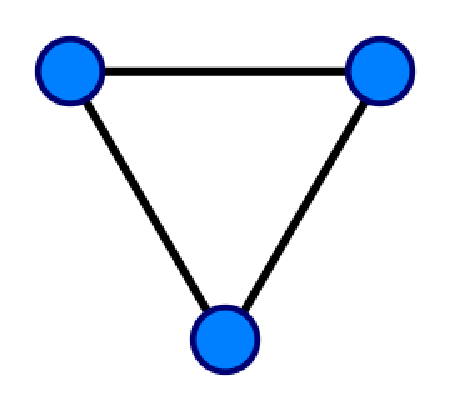
\includegraphics[width=0.25\textwidth]{abb/misc/GraphBsp.eps}
	\caption[Ungerichteres Netzwerk]{Beispiel eines ungerichteten Netzwerks aus vier Knoten, bei dem jeder Knoten mit jedem anderen verbunden ist.}
	\label{fig:GraphBsp}
\end{figure}


\subsection*{Dynamik auf Netzwerken}
Um Prozesse auf Netzwerken zu beschreiben kann man jedem Knoten eine $n$-dimensionale dynamische Variable $x_i$ zuordnen. Die Dynamik wird dann für jeden Knoten über eine Differentialgleichung beschrieben, die die Kopplung an die anderen Knoten enthält. Die allgemeine Form dieser Differentialgleichung ist in Gleichung (\ref*{eq:dyneqcommon}) gezeigt.

%was ist das mit der rückkopplung? die ist doch da drin? haben wir mal rausgenommen

\begin{align}\label{eq:dyneqcommon}
\overset{\cdot}{\boldsymbol{x}}_i(t)&=\boldsymbol{f}(\boldsymbol{x}_i(t))+\sigma\sum_j A_{ij}\boldsymbol{h}\left(\boldsymbol{x}_j(t)\right)
\\\notag & i=1,...,N
\\\notag & \sigma \text{ allgemeine Kopplungsstärke}
\\\notag & A_{ij}\text{ Element der Kopplungsmatrix}
\\\notag & \boldsymbol{f},\boldsymbol{h}:\mathbb{R}^n\rightarrow\mathbb{R}^n
\end{align}
Die Verbindungsmatrix $\boldsymbol{A}$ wird hierbei zu einer Kopplungsmatrix, die die Kopplung der Differentialgleichungen der Knoten untereinander beschreibt. Im folgenden werden nur solche Systeme betrachtete, bei denen $\boldsymbol{A}$ symmetrisch ist, das Netzwerk also ungerichtet. Die Abbildung $\boldsymbol{h}$ beschreibt auf welche Art und Weise die Komponenten der Variablen $\boldsymbol{x}_i$ aneinander koppeln. Das Differentialgleichungssystem in (\ref*{eq:dyneqcommon}) lässt sich auch über das Kronecker-Produkt in einer einzigen Gleichung darstellen \citep{pecora1998},
\begin{align}
\overset{\cdot}{\boldsymbol{X}}(t)=\boldsymbol{F}(\boldsymbol{X}(t))+\sigma\boldsymbol{A}\otimes\boldsymbol{H}(\boldsymbol{X}(t))
\end{align}
mit den Definitionen:
\begin{align*}
\boldsymbol{X}=\left(\boldsymbol{x}_1,...,\boldsymbol{x}_N\right)^{\text{T}},
\boldsymbol{F}=\left(\boldsymbol{f}(\boldsymbol{x}_1),...,\boldsymbol{f}(\boldsymbol{x}_N)\right)^{\text{T}},
\boldsymbol{H}=\left(\boldsymbol{h}(\boldsymbol{x}_1),...,\boldsymbol{h}(\boldsymbol{x}_N)\right)^{\text{T}}
\end{align*}



\section{Synchronisation}
\subsection*{Globale Synchronisation}
Das Netzwerk wird als global synchron bezeichnet, wenn sich alle Variablen $\boldsymbol{x}_i$ zeitlich gleich verhalten.
\begin{align*}
\boldsymbol{x}_1(t)=\boldsymbol{x}_2(t)=...=\boldsymbol{x}_N(t)=:\boldsymbol{s}(t)
\end{align*}
Es spielt dabei keine Rolle, ob dieses Verhalten z.B konstant, periodisch oder chaotisch ist.

\subsection*{Isolierte Synchronisation}
Isolierte Synchronisation liegt vor, wenn eine Gruppe von Knoten oben genanntes Verhalten aufweist, während ein anderer Teil des Netzwerks nicht synchron mit dieser Gruppe ist.



\section{Stabilität der Synchronisation}
Ein synchroner Zustand eines Netzwerks lässt sich hinsichtlicht seiner Stabilität untersuchen. Dabei wird eine kleine Abweichung $\boldsymbol{x}_i(t)$ der Anfangsbedingungen des synchronen Zustandes angenommen und berechnet, wie sich diese Störung zeitlich weiterentwickelt.
\begin{align}\label{eq:deltaxi}
\delta \boldsymbol{x}_i(t) &= \boldsymbol{x}_i - \boldsymbol{s}(t)\\
\delta \overset{\cdot}{\boldsymbol{x}}_i(t) &= \boldsymbol{f}(\boldsymbol{x}_i(t))+\sigma\sum_j A_{ij}\boldsymbol{h}\left(\boldsymbol{x}_j(t)\right) - \overset{\cdot}{\boldsymbol{s}}(t)
\end{align}
Eine Linearisierung dieser Gleichung um die Bahnkurve $\boldsymbol{s}(t)$ liefert in der Kronecker-Produkt Schreibweise die Master Stability Equation (MSE) in Gleichung (\ref*{eq:mse}).
\begin{align}\label{eq:mse}
\delta\overset{\cdot}{\boldsymbol{X}}(t)=
\left[D\boldsymbol{F}(\boldsymbol{s}(t))+\sigma\boldsymbol{A}\otimes D\boldsymbol{H}(\boldsymbol{s}(t))\right]\delta\boldsymbol{X}(t)
\end{align}

\subsection*{Ljapunow-Exponenten}
Die Ljapunow-Exponenten beschreiben, wie weit sich Bahnkurven für große Zeiten von einander entfernen, verglichen mit der Abweichung zum Zeitpunkt $t=0$. Eine mögliche Definition ist in Gleichung (\ref{eq:ljapunow}) gegeben.
\begin{align}\label{eq:ljapunow}
\lambda_i=\lim_{t\rightarrow\infty}\frac{1}{t} ln\left(\frac{|\delta \boldsymbol{x}_i(t)|}{|\delta \boldsymbol{x}_i(0)|}\right)
\end{align}
Wird die Abweichung zu $\delta\boldsymbol{x}_i(0)$ größer, so ist der Quotient größer als 1, sonst kleiner. Es gilt also folgende Unterscheidung für die Werte der Ljapunow-Exponenten.
\begin{equation}
\begin{cases}
\lambda_i < 0, \text{ Abweichung vom synchronen Zustand verschwindet}\\
\lambda_i > 0, \text{ Abweichung vom synchronen Zustand wächst}
\end{cases}
\end{equation}
Positive Ljapunow-Exponenten weisen eine instabile Synchronisation nach und negative eine stabile. Der Stabilitätsbegriff bezieht sich hierbei auf Invarianz der Bahnkurven gegenüber Änderungen der Anfangsbedingungen (für lange Zeiten). 
\subsection*{Master Stability Function}
Durch eine Diagonalisierung der Kopplungsmatrix lässt sich bei Betrachtung entlang ihrer Eigenvektoren die Kopplungsmatrix in (\ref{eq:mse}) durch ihre Eigenwerte $\alpha+i\beta$ darstellen. In dieser Form lassen sich die Ljapunow-Exponenten zu den Richtungen transversal zur Synchronisation berechnen. Da es für Instabilität genügt, wenn einer dieser Ljapunow-Exponenten größer als 0 ist, ist es sinnvoll nur den größten zu betrachten. Dieser wird Master Stability Function (MSF) gennant. 





\section{Symmetrien}
Können in einem Graphen zwei Knoten miteinander vertauscht werden, ohne dass sich der Graph verändert, liegt eine Permutationssymmetrie vor \cite{symmetrie}. Für die betrachteten Netzwerke bedeutet dies, dass sich bei Vorliegen einer Permutationssymmetrie zwei Knoten tauschen lassen, indem sowohl die zugehörigen Spalten als auch Zeilen der Kopplungsmatrix getauscht werden, ohne dass sich die Dynamik des Systems verändert. Die Vertauschung der Knoten lässt sich durch eine Permutationsmatrix $P$ darstellen. Vorraussetzung für eine Permutationssymmetrie ist somit\cite{pecora2014}
\begin{equation}
PAP^{-1}=A.
\end{equation}

Zur Untersuchung eines Netzwerkes auf Symmetrien, eignet sich die Suche von Automorphismen des dem Netzwerk zugrunde liegenden Graphen mit Hilfe der Bibliothek \textit{nauty} \cite{nauty}. Mit dieser lassen sich neben den Generatoren der Permutationssymmetrien, auch die Orbits der Knoten bestimmen. Als Orbit werden hierbei die Positionen bezeichnet, an die ein Knoten durch Anwendung aller Permutationen gelangen kann. Alle Knoten eines Orbits lassen sich folglich durch eine Hintereinaderreihung der Permutationen vertauschen, ohne dass sich die Dynamik des Netzwerkes verändert. Eine solche Gruppe von Knoten wird als Cluster bezeichnet. Sollte bei der für die Vertauschung nötigen Hintereinanderreihung von Permutationen ebenfalls Knoten eines weiteren Clusters miteinander vertauscht werden, so liegt eine Verschränkung der Cluster vor (interwinded Clusters)\cite{pecora2014}.

\section{Synchronisation in symmetrischen Netzwerken}
Da Knoten eines Clusters ohne Veränderung der Dynamik vertauschbar sind, erhalten diese den gleichen Input der anderen Knoten und können synchron laufen. In einem aus M Clustern $C_m$ bestehenden Netzwerk existieren somit M Gruppen von Knoten, die isolierte Synchronisation aufweisen können mit synchronen Orbits $s_m$
\begin{equation}
x_i(t)=s_m(t) \text{ mit } \textit{Knoten } i\in C_m.
\end{equation}

{\subsection*{Isolierte Desynchronisation}}
In einem symmetrischen Netzwerk können einzelne Cluster synchron sein, während andere nicht synchron sind. Die Desynchronisation scheint also die Synchronisation eines anderen Clusters nicht zwangsläufig zu stören\cite{pecora2014}.

Unter einer Permutation $\pi$, eines Clusters A, mit Permutationsmatrix $P_A$, ändert sich die Dynamik eines Knotens $i$ aus einem disjunkten Cluster B nicht, es gilt



\begin{align}
		\notag \left[\boldsymbol{P}_A	\overset{\cdot}{\boldsymbol{X}}\right]_i&= \overset{\cdot}{\boldsymbol{x}}_i\\
		\notag\left[\boldsymbol{P}_A \boldsymbol{F}(\boldsymbol{X})\right]_i+
			\left[\boldsymbol{P}_A\boldsymbol{A}\boldsymbol{H}(\boldsymbol{X})\right]_i&=
			\boldsymbol{f}(\boldsymbol{x}_i)+
			\sigma\sum_j A_{ij}\boldsymbol{h}(\boldsymbol{x}_j)\\
		\boldsymbol{f}(\boldsymbol{x}_i)+
			\sigma\sum_j A_{ij}\boldsymbol{h}(\boldsymbol{x}_{\pi\left(j\right)})&=
		\boldsymbol{f}(\boldsymbol{x}_i)+
			\sigma\sum_j A_{ij}\boldsymbol{h}(\boldsymbol{x}_j)		
\end{align}
Folglich muss jeder Knoten in A gleich an den Knoten $i$ gekoppelt sein und dieser somit gleichstarken Input von allen Knoten aus A erhalten (siehe Abb. \ref{fig:perma}).

\begin{figure}
		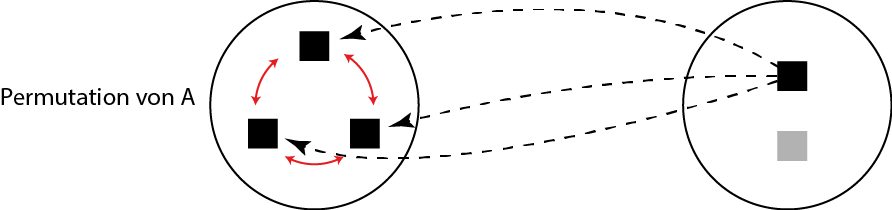
\includegraphics[width=0.75\textwidth]{abb/misc/perm_a.png}
		\caption{Es werden zwei Cluster A und B betrachtet. Eine Symmetriepermutation des Clusters A ändert die Dynamik eines Knotens in B nicht. Folglich muss dieser Knoten gleichstarken Input von jedem Knoten aus A erhalten.}
		\label{fig:perma}
\end{figure}


Eine analoge Betrachtung  unter Permutation des den Knoten $i$ enthaltenden Clusters B (A wird nicht verändert) führt auf die Beobachtung, dass jeder Knoten aus B gleich an die Knoten aus A gekoppelt ist (siehe Abb. \ref{fig:permb}). 

Zusammen ergibt sich aus diesen Aussagen: Jeder Knoten in B bekommt in der Summe den gleichen Input vom Cluster A, egal ob dieser synchron oder asynchron ist, sofern Permutationsmatrizen existieren, die die Cluster getrennt permutieren. Isolierte Desynchronisation kann nicht bei "verschränkten" Clustern auftreten, da die Permutation beide Cluster verändert.

	\begin{figure}
		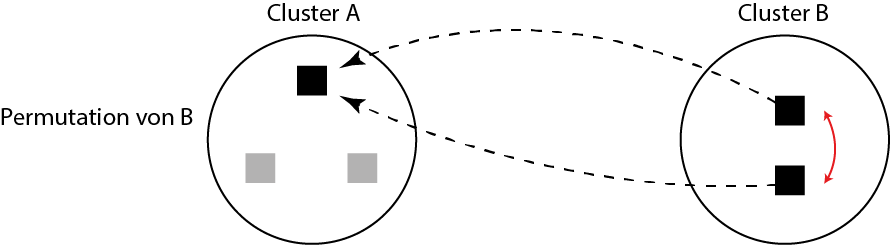
\includegraphics[width=0.75\textwidth]{abb/misc/perm_b.png}
		\caption{Bei Symmetriepermutation des Clusters B ändert sich die Dynamik eines Knotens aus B nicht. Somit muss jeder Knoten aus B gleichstarken Input von A erhalten.}
		\label{fig:permb}
	\end{figure}
	

\subsection*{Stabilität}
\label{stabilitaet}
Zur Betrachtung der Stabilität der isolierten Synchronisation lässt sich die MSE (\ref{eq:mse})  unter Verwendung von Clustermatrizen $\boldsymbol{E^m}$ (beschreiben die Zuordnung der Knoten zu den Clustern)
\begin{align}
 \boldsymbol{E}^{(m)}_{ii} =1\text{ wenn Knoten }i \in C_m.
\end{align}
 umschreiben zu\cite{pecora2014}:
\begin{align}
	\label{eq:clustermse}
\notag	\delta\overset{\cdot}{\boldsymbol{X}}(t)&=	
	\left[D\boldsymbol{F}(\boldsymbol{s}(t))+\sigma\boldsymbol{A}\otimes D\boldsymbol{H}(\boldsymbol{s}(t))\right]\delta\boldsymbol{X}(t)\\&=
	\left[\sum_{m=1}^{M} \boldsymbol{E}^{(m)} \otimes D\boldsymbol{F}(\boldsymbol{s}_m(t))+\sigma\boldsymbol{A}\otimes \boldsymbol{I}_n\sum_{m=1}^{M} 			\boldsymbol{E}^{(m)}\otimes D\boldsymbol{H}(\boldsymbol{s}_m(t))\right]\boldsymbol{X}(t)
	\end{align}
	
Gleichung (\ref{eq:clustermse}) lässt sich mithilfe der Gruppentheorie in eine neue Basis transformieren\cite{pecora2014}. Hierbei wird die Basis der irreduziblen Darstellungen (IRR), der den Permutationssymmetrien zugrundeliegenden Gruppe gewählt. In dieser Basis nimmt die Kopplungsmatrix Blockdiagonalform an. Die oberen M Koordinaten $\eta(t)$ in der neuen Darstellung entsprechen einer Bewegung longitudinal innerhalb der Synchronisationsmannigfaltigkeit, die weiteren einer Bewegung transversal zur ihr. Die Transformationsmatrix $\boldsymbol{T}$ lässt sich mit einer geeigneten Software für diskrete Mathematik (z.B. sage) bestimmen \citep{sagenotebook}. Diese Basistransformation entspricht einer Transformation in $M$ Schwerpunktkoordinaten und $(N-M)$ Relativkoordinaten (die die Abweichung der Knoten eines Clusters zueinander beschreiben) mit orthogonalen Basisvektoren.
Aus der so transformierten MSE (\ref{eq:irrmse}) lässt sich die MSF berechnen um die Stabilität der Clustersynchronisation zu beurteilen,
\begin{align}
	\label{eq:irrmse}
		\overset{\cdot}{\boldsymbol{\eta}}(t)&=
				\left[\sum_{m=1}^{M} \boldsymbol{J}^{(m)} \otimes D\boldsymbol{F}(\boldsymbol{s}_m(t))+\sigma\boldsymbol{B}\otimes \boldsymbol{I}_n\sum_{m=1}^{M} \boldsymbol{J}^{(m)}\otimes D\boldsymbol{H}(\boldsymbol{s}_m(t))\right]\boldsymbol{\eta}(t)
		\end{align}
		mit der transformierten Kopplungsmatrix $\boldsymbol{B}$ und den transformierten Clustermatrizen $\boldsymbol{J}^{(m)}$
		\begin{align}
				 \boldsymbol{\eta}(t)&=\boldsymbol{T}\otimes\boldsymbol{I}_n\delta\boldsymbol{X}(t)
				\\\notag \boldsymbol{B}&=\boldsymbol{T}\boldsymbol{A}\boldsymbol{T}^{-1}
				\\\notag \boldsymbol{J}^{(m)}&=\boldsymbol{T}\boldsymbol{E}^{(m)}\boldsymbol{T}^{-1}.
		\end{align}
		






\section{Simulationsbeispiel}
Die vorgestellten Methoden zur lokalen Stabilitätsanalyse eines Netzwerks werden in diesem Abschnitt auf ein Beispiel angewendet. Bisher wurden nur dynamische Systeme mit kontinuierlichen Variablen betrachtet. Die zugrunde liegende Theorie lässt sich auch auf diskrete Systeme anwenden. Dabei ist die Dynamik nicht durch ein Differentialgleichungssystem gegeben, sondern durch eine Iterationsvorschrift. Das hier betrachtete Netzwerk \cite{pecora2014} folgt der Dynamik in Gleichung (\ref{eq:bspdyn}).
\begin{align}
\label{eq:bspdyn}
	x_i^{t+1}&=\left[\beta\mathcal{I}(x_i^t)+\sigma \sum_j^N A_{ij}\mathcal{I}(x_j^t)+\delta\right] \text{mod}\quad 2\pi
	\\\notag & \beta,\sigma \text{ Kopplungsparameter}
	\\\notag  & \delta \text{ Offset}
	\\\notag &\mathcal{I}(x)=\frac{1-Cos(x)}{2}
\end{align}
Die betrachteten Netzwerke sind symmetrisch und bestehen aus $N=11$ Knoten. Die verwendeten Kopplungsmatrizen (\ref{Amat}) sind Pecora et al. \cite{pecora2014} entnommen. Eines der betrachteten Netwerke ist exemplarisch in Abb. \ref{fig:cluster}, die zugehörige Kopplungsmatrix in Abb. \ref{fig:abmat} dargestellt. 
\begin{figure}
	 \centering
	 \subfloat[Netzwerk 1]{
	 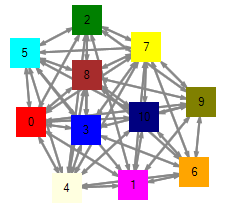
\includegraphics[width=0.25\textwidth]{abb/misc/cluster1.png}
	 }
	 \subfloat[Netzwerk 2]{
	 	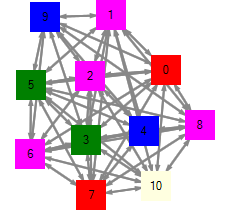
\includegraphics[width=0.25\textwidth]{abb/misc/cluster2.png}
	 }
	 \subfloat[Netzwerk 3]{
	 	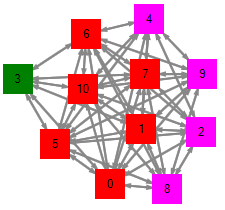
\includegraphics[width=0.25\textwidth]{abb/misc/cluster3.png}
	 }
	 \caption[In der Simulation verwendete Netzwerke]{Die drei verwendeten Netzwerke. Die Knoten eines Cluster sind in der gleichen Farbe eingefärbt.}
	 \label{fig:cluster}
\end{figure}

\begin{figure}
	\centering
	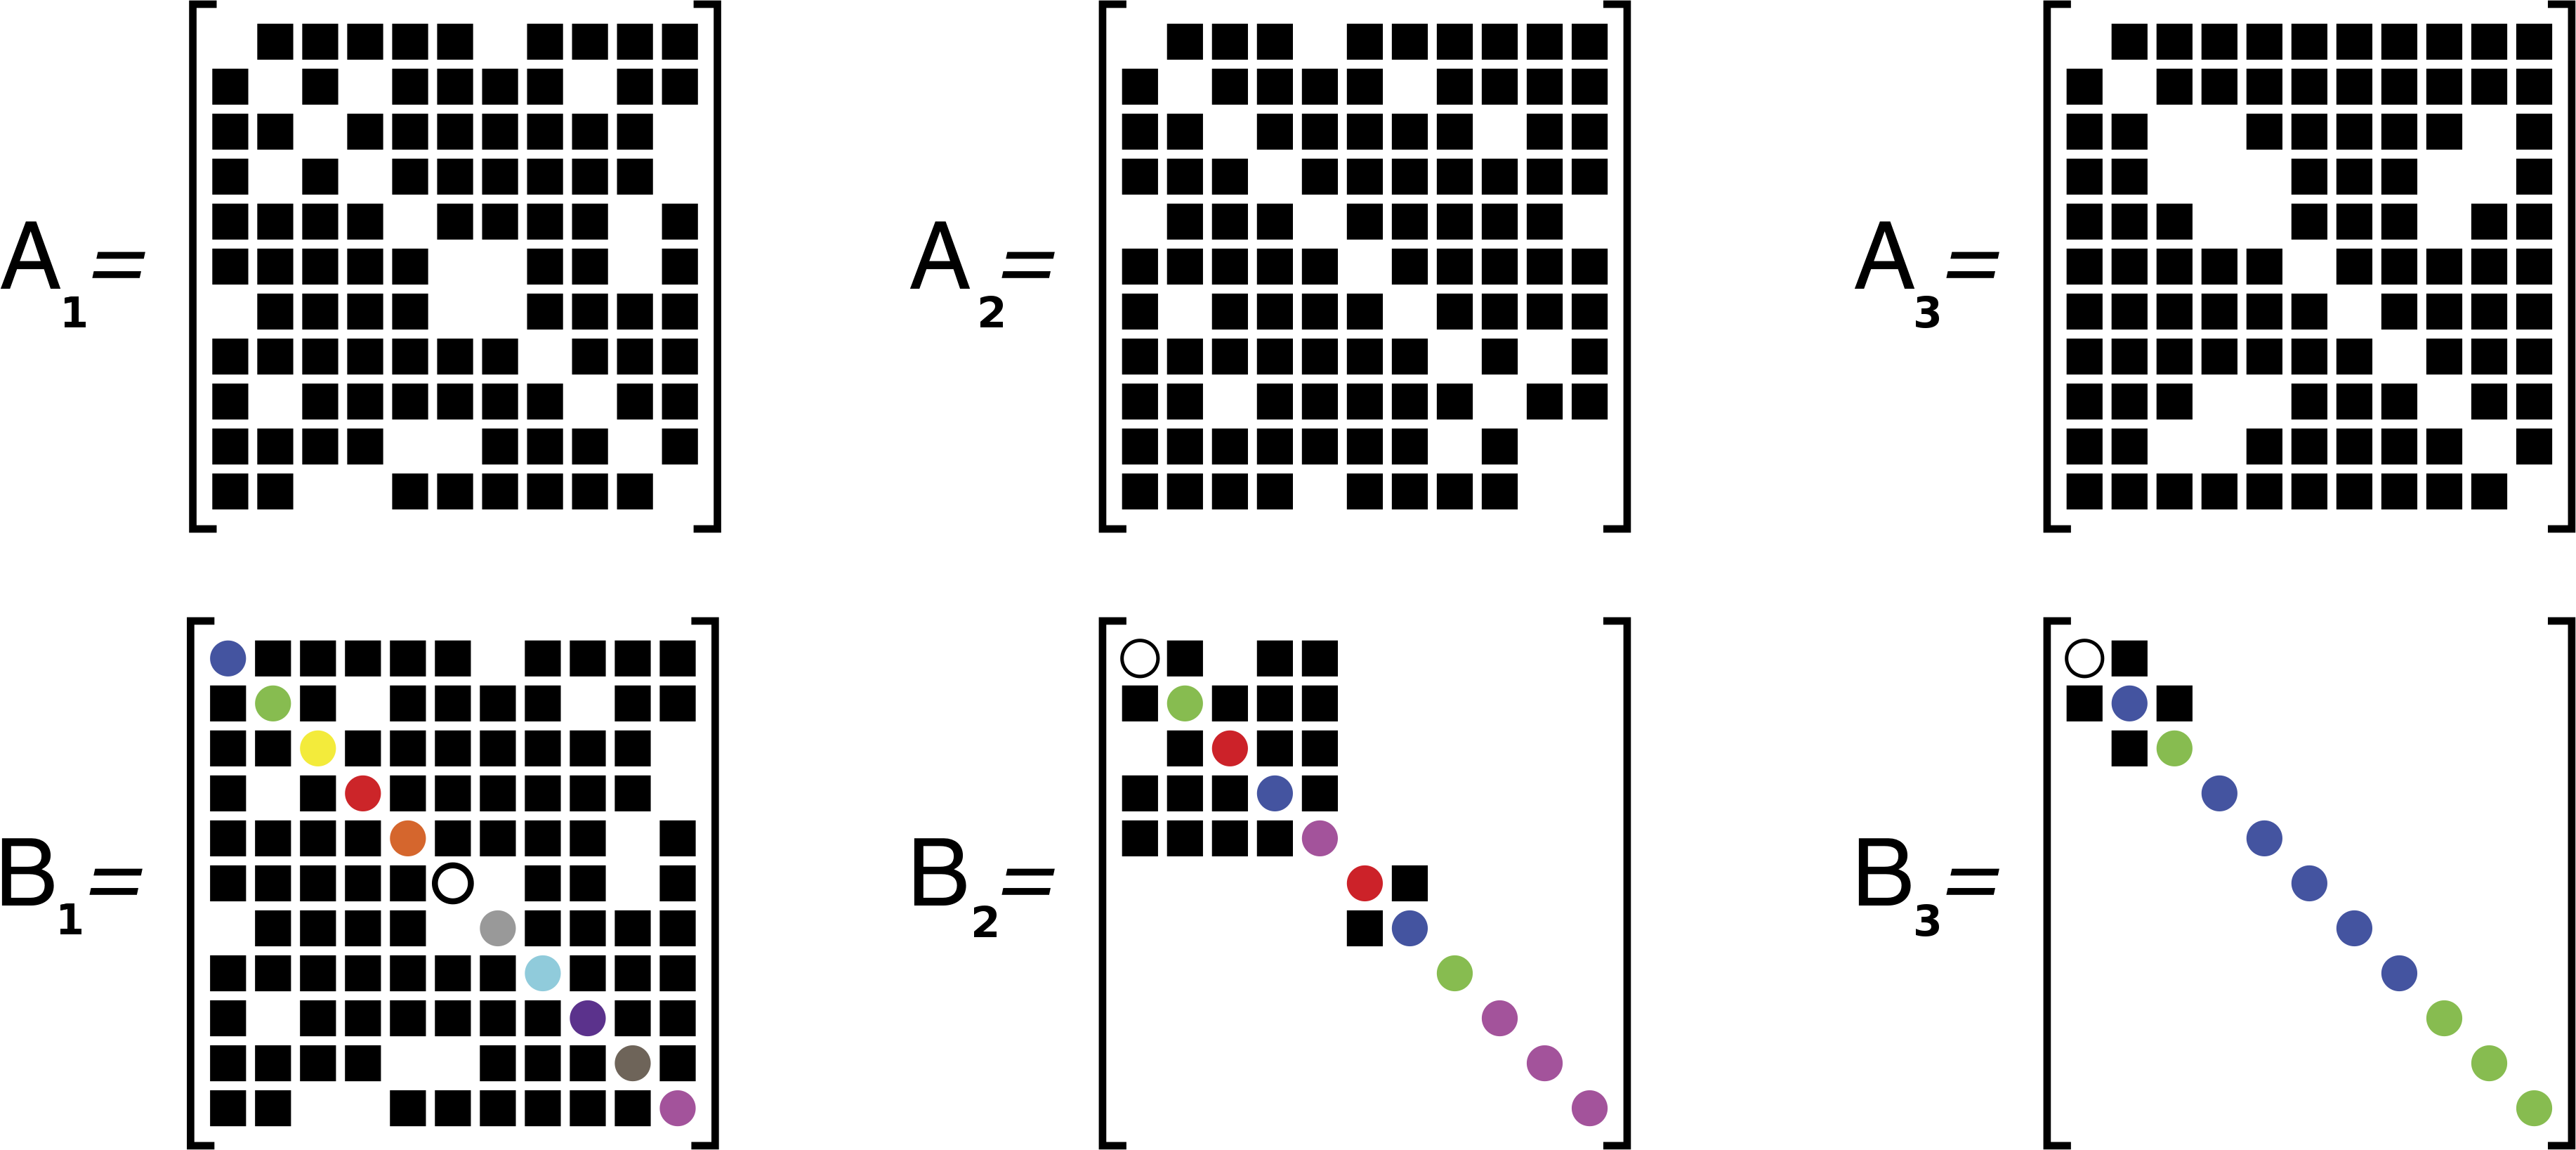
\includegraphics[width=0.5\textwidth]{abb/misc/ABMat.png}
	\caption[Kopplungsmatritzen und ihre Transformierten]{Kopplungsmatrizen $\boldsymbol{A}$ der in Abb. \ref{fig:cluster} dargestellten Netwerke sowie die transformierten Kopplungsmatrizen $\boldsymbol{B}$ in der die Zeilen nach den zugehörigen Clustern markiert sind\cite{pecora2014}.}
\label{fig:abmat}
\end{figure}

In diesen Netwerken ergibt die Clustersuche mit Nauty..


-bild vom netzwerk

-cluster, anzahl symmetrien

-rms

Zur Berechnung der Ljaponow-Exponenten wurde eine Basistransformation (siehe \ref{stabilitaet}) mit den im Anhang (\ref{Tmat}) dargestellten Transformationsmatrizen vorgenommen \cite{pecora2014,sagenotebook}
-ljapunow



\section{Fazit}\label{fazit}
Die Existenz von synchronisierenden Clustern in einem Netzwerk ergibt sich aus vorhandenen Symmetrien des Netzwerkes. Das Phänomen der isolierten Synchronisation einzelner Cluster lässt sich über die Betrachtung der Dynamik unter Symmetriepermutationen erklären. 
Die Master Stability Function ist ein bekanntes Hilfsmittel um die globale Synchronisation in Netzwerken hinsichtlich der Stabilität zu analysieren. Durch eine Basistransformation können mit der MSF darüber hinaus Aussagen über die Stabilität der lokalen Synchronisation innerhalb der Cluster getroffen werden.\\
Anhand eines Simulationsbeispiels wurden verschiedene Netzwerke mit diskreter Dynamik auf Permutationssymmetrien untersucht, darüber die vorhandenen Cluster identifiziert und die vorgestellte Methode zur Analyse der Stabilität der Synchronisation verifiziert.


%% Beispiel für Bild mit Fußnote
\begin{figure}[htb]
 \centering
 \includegraphics[width=0.4\textwidth,angle=45]{abb/logo1}
 \caption[Beispiel einer Bildbeschreibung]{Beispiel einer Bildbeschreibung\footnotemark}
\label{fig:beispiel1}
\end{figure}
\footnotetext{Bildquelle: Beispielquelle}

% Beispiel für Bildintegration
\begin{figure}[htb]
 \centering
 \includegraphics[width=0.3\textwidth,angle=0]{abb/logo2}
 \caption[Beschreibung]{Beschreibung}
\label{fig:Beschreibung}
\end{figure}

% Beispiel: Referenz auf Abbildung
Abbildung~\ref{fig:Beschreibung} [S.\pageref{fig:Beschreibung}]

% Beispiel: Tabelle 
\begin{center}
  \begin{tabular}{ | l | c | }
    \hline
    Überschrift 1 & Überschrift 2 \\ \hline \hline
    Info 1 & Info 2 \\ \hline
    Info 3 & Info 4 \\
    \hline
  \end{tabular}
\end{center}


% Beispiel für Quellcode Listings
\lstset{language=xml}
\begin{lstlisting}[frame=htrbl, caption={Die Datei {\tt data-config.xml} dient als Beispiel für XML Quellcode}, label={lst:dataconfigxml}]
<dataConfig>
  <dataSource type="JdbcDataSource" 
              driver="com.mysql.jdbc.Driver"
              url="jdbc:mysql://localhost/bms_db"
              user="root" 
              password=""/>
  <document>
    <entity name="id"
        query="select id, htmlBody, sentDate, sentFrom, subject, textBody
        from mail">
    <field column="id" name="id"/>
    <field column="htmlBody" name="text"/>
    <field column="sentDate" name="sentDate"/>
    <field column="sentFrom" name="sentFrom"/>
    <field column="subject"  name="subject"/>
    <field column="textBody" name="text"/>
    </entity>
  </document>
</dataConfig>
\end{lstlisting}

\lstset{language=java}
\begin{lstlisting}[frame=htrbl, caption={Das Listing zeigt Java Quellcode}, label={lst:result2}]
/* generate TagCloud */
Cloud cloud = new Cloud();
cloud.setMaxWeight(_maxSizeOfText);
cloud.setMinWeight(_minSizeOfText);
cloud.setTagCase(Case.LOWER);
	    
/* evaluate context and find additional stopwords */
String query = getContextQuery(_context);
List<String> contextStoplist = new ArrayList<String>();
contextStoplist = getStopwordsFromDB(query);
	    
/* append context stoplist */
while(contextStoplist != null && !contextStoplist.isEmpty())
  _stoplist.add(contextStoplist.remove(0));
	    
/* add cloud filters */
if (_stoplist != null) {
  DictionaryFilter df = new DictionaryFilter(_stoplist);
  cloud.addInputFilter(df);
}
/* remove empty tags */
NonNullFilter<Tag> nnf = new NonNullFilter<Tag>();
cloud.addInputFilter(nnf);

/* set minimum tag length */
MinLengthFilter mlf = new MinLengthFilter(_minTagLength);
cloud.addInputFilter(mlf);

/* add taglist to tagcloud */
cloud.addText(_taglist);

/* set number of shown tags */	    
cloud.setMaxTagsToDisplay(_tagsToDisplay);
\end{lstlisting}


% Beispiel für Formeln
Die Zuordnung aller möglichen Werte, welche eine Zufallsvariable annehmen kann nennt man \emph{Verteilungsfunktion} von $X$.

\begin{quotation}
Die Funktion F: $\mathbb{R} \rightarrow$ [0,1] mit $F(t) = P (X \le t)$ heißt Verteilungsfunktion von $X$.\footnote{Konen, vgl.~\cite{wk05}~[S.55]}
\end{quotation}

\begin{quotation}
Für eine stetige Zufallsvariable $X: \Omega \rightarrow \mathbb{R}$ heißt eine integrierbare, nichtnegative reelle Funktion $w: \mathbb{R} \rightarrow \mathbb{R}$ mit $F(x) = P(X \le x) = \int_{-\infty}^{x} w(t)dt$ die \emph{Dichte} oder \emph{Wahrscheinlichkeitsdichte} der Zufallsvariablen $X$.\footnote{Konen, vgl.~\cite{wk05}~[S.56]}
\end{quotation}


\onecolumn
% einfacher Zeilenabstand
\singlespacing
% Literaturliste soll im Inhaltsverzeichnis auftauchen
\newpage
\addcontentsline{toc}{section}{Literaturverzeichnis}
% Literaturverzeichnis anzeigen
\renewcommand\refname{Literaturverzeichnis}

\bibliography{Hauptdatei}

%% Index soll Stichwortverzeichnis heissen
% \newpage
% % Stichwortverzeichnis soll im Inhaltsverzeichnis auftauchen
% \addcontentsline{toc}{section}{Stichwortverzeichnis}
% \renewcommand{\indexname}{Stichwortverzeichnis}
% % Stichwortverzeichnis endgueltig anzeigen
% \printindex

\onehalfspacing
% evtl. Anhang
\newpage
\addcontentsline{toc}{section}{Anhang}
\fancyhead[L]{Anhang} %Kopfzeile links
\subsection*{Anhang}\label{anhang}




% leere Abschlussseite
%\newpage
%\thispagestyle{empty} % erzeugt Seite ohne Kopf- / Fusszeile
%\section*{ }

\end{document}\grid
